As the goal of a hydrogel scaffold is to promote natural healing, it must degrade over time to
allow the naturally-formed tissue to take over, yet its lifespan must be long enough to
continuously support the afflicted area throughout the healing process. Tendon and ligament
repair is a lengthy process that can take several months to over a year for full healing \autocite{RN1}. Traditional polymer-based hydrogels degrade too quickly to be effective in long healing
processes. Depending on the specific chemical composition, these hydrogels can degrade
within the body in less than 6 months due to hydrolysis, oxidization, and enzymatic activity.
Therefore, the use of a composite hydrogel becomes absolutely necessary for use in
tendon/ligament repair.

Composite hydrogels incorporate blends of natural and synthetic materials and linkage
structures such as double networks and interpenetrating networks. These hydrogels not only
last longer than natural or synthetic polymer-based hydrogels, but are also tunable, as their
lifespan can be modified by adjusting the cross-linking type and density. This allows for
improved customizability while maintaining permeability and resisting premature degradation. In
addition, the hydrogel structure can be engineered to respond to environmental stimuli such as
pH and enzyme presence, allowing them to be dynamic and responsive to the state of the
healing tissue, gradually breaking down in sync with tissue regeneration \autocite{RN3}.

\subsection{Effects of Crosslinking on Hydrogel Degradation
}

As mentioned above, composite hydrogels are highly customizable. Their lifespan may be
customized to better fit the timeline of the specific injury being treated. One such technique is
modifying the crosslinking density between hydrogel layers. A study by \autocite{RN4} found that an
increased concentration of glutaraldehyde crosslinking correlates with higher mechanical
strength and lower degradation rates. Greater crosslinking forms a denser polymer network,
making the hydrogel more resistant to breakdown from oxidation, hydrolysis, and enzymatic
activity (\citeyear{RN4}).

\subsection{Degradation of the JTA}

% Figure for Self-Healing,
% need to include here for correct positioning
\begin{figure*}[b]
    \centering 
    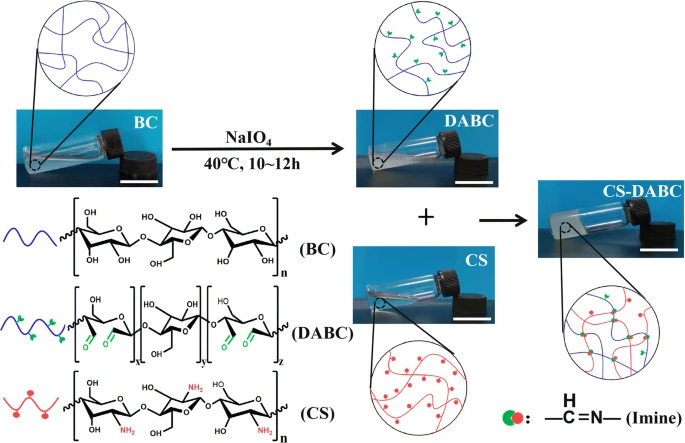
\includegraphics[width=0.7\linewidth]{Figures/CS_DABC_condensation.jpg}
    \caption{Schematic representation of hydrogel synthesis from chitosan and dialdehyde bacterial cellulose \autocite{liAllnaturalInjectableHydrogel2020}}
    \label{fig:CS_DABC_condensation}
\end{figure*}

The JTA combines several natural and synthetic materials, all of which must be safely broken down within the body to serve as an effective treatment. Alginate, a water-soluble polysaccharide which makes up the hydrophilic matrix of the hydrogel, degrades into monosaccharides, primarily guluronic and mannuronic acid units. These are very easily excreted from the body via the renal system. 
Chitosan, a cationic polymer typically used in the bioadhesive layer of the JTA, degrades into glucosamine and N-acetylglucosamine. These monosaccharides are involved in the body's natural metabolic processes, so they are very easily reintegrated into the body's metabolic system following the breakdown of the JTA \autocite{guarinoDegradationPropertiesMetabolic2015}.
Polyacrylamide, a synthetic polymer that makes up the backbone of the double-network structure, breaks down into acrylamide monomers. These synthetic byproducts can either be metabolized by the liver before being excreted via urine, or they can undergo conjugation with glutathione or glutathione-S-transferases, making them non-toxic and water-soluble \autocite{xiongPolyacrylamideDegradationIts2018}.
Schiff base linkages, which provide dynamic crosslinking within the JTA, hydrolyze into aldehydes and amines, which are non-toxic and easily metabolized or excreted \autocite{xuHydrogelsBasedSchiff2019}.

The degradation process roughly follows in the following order, from quickest to slowest degradation: alginate, chitosan, imine bonds, polyacrylamide. This order is very beneficial for the healing process. Alginate and chitosan, being natural components of the hydrogel, degrade quickly within the body, softening the scaffold slightly.
This both increases the permeability of the scaffold, allowing cells and nutrients to enter and exit more efficiently, and encourages integration of the healing tissues with the hydrogel scaffold \autocite{RN4}.
Imine bonds provide the self-healing factor of the JTA, allowing it to recover from minor deformations and maintain structural integrity under movement. However, these bonds also degrade over time, after about 1-3 months, allowing more mechanical load to be gradually shifted from the scaffold onto the recovering tissue \autocite{xuHydrogelsBasedSchiff2019}.
The polyacrylamide backbone, being a synthetic polymer, is the last to degrade within the body. This structure is critical in providing support to the tissue and must degrade approximately synchronously with the recovery time of the injury.